\documentclass[10pt,a4paper]{article}
\usepackage[margin=2.2cm]{geometry}
\usepackage{fontspec}
\usepackage{amsmath,amssymb}
\usepackage{booktabs,graphicx,float,xcolor,array}
\usepackage[font=small,labelfont=bf]{caption}
\usepackage{enumitem}
\usepackage[colorlinks=true,linkcolor=blue!50!black,urlcolor=blue!50!black,citecolor=blue!50!black]{hyperref}
\setlist{itemsep=2pt,topsep=3pt}
\graphicspath{{../figures/round3/}{../figures/round4/}}
\newcommand{\tabthree}[1]{\IfFileExists{tables_r3/#1.tex}{\input{tables_r3/#1.tex}}{}}
\newcommand{\tabfour}[1]{\IfFileExists{tables_r4/#1.tex}{\input{tables_r4/#1.tex}}{}}
\newcommand{\code}[1]{\texttt{#1}}

\title{\textbf{Scaling NBN, rounds 3 and 4: does a larger budget buy a better answer?}\\[4pt]
\large Threads, GPU, memory and time; conditioning, anytime certified sampling, bounded conditioning}
\author{Alfredo (\code{alfredo\_claude}) for Giovanni Briglia}
\date{17 October 2026 --- branch \code{feat/scaling-mechanisms}, local, not pushed}

\begin{document}
\maketitle

\section*{Summary}
\textbf{Question.} If NBN gets more workers (threads, a GPU), more memory or more time, does it
give a better answer? \textbf{Round 3} measured this on the existing methods. \textbf{Round 4}
adds three opt-in options so that exact and certified inference can also use a larger budget.
Defaults and semantics are unchanged.
\begin{itemize}
\item \textbf{Before (round 3).} Sampling, fitting and amortized methods use a larger budget: a
$4\times$ budget moves the largest graph finished by 2--$10\times$, and LW error falls like
$1/\sqrt{\text{particles}}$. Exact VE does not: its limit is the elimination width, and $4\times$
memory adds only $\log_3 4\approx1.26$ to it ($16\to17$). Time could not help VE at all.
\item \textbf{Conditioning (round 4, change 1).} Exact answers when VE does not fit. All 40
conditioned answers that have a VE reference match it to $1.7\cdot10^{-7}$. At 1\,GB on the
degree-3 graphs, plain VE answers 6/10 queries (0/10 on MPS); conditioning answers 8--10/10.
Workers now divide the time of an exact answer: for the same query, 20 CPU threads are about
$5\times$ faster than 1 thread, and the TITAN X 30--$100\times$.
\item \textbf{Anytime certified sampling (change 2).} Stop on time or on a target width with a
valid 95\% interval; the width falls like $1/\sqrt{t}$, and every interval covered the exact
answer (584/584 runs where the exact answer is known). Collapsed sampling (\code{collapse="auto"}) returns the exact answer when the
query fits, and helps on the GPU; on CPU it is slower than plain sampling on dense graphs.
\item \textbf{Bounded conditioning (change 3).} Sound bounds with no probability, exact at the
end. In practice they stay near $[0,1]$ on these networks: with evidence, the unseen prior mass
dwarfs $P(e)$. An honest negative result; a tighter bound is sketched in §\ref{sec:next}.
\item \textbf{Hard limit.} At average degree $\ge4.5$ the cutsets have 10--24 variables
($3^{10}$--$3^{24}$ instantiations): exact answers would need $10^3$--$10^7$\,s even on the GPU.
There, only sampling answers, and the certified interval is the honest output.
\end{itemize}

\section{The question and what theory predicts}
A budget has three parts: \emph{workers} (CPU threads, a GPU), \emph{memory} and \emph{time}.
A method ``scales with the budget'' if a larger budget gives a faster answer, a larger model, or a
better answer. The experts (\code{koller\_claude}: Koller \& Friedman 2009; \code{moss\_claude}:
Kochenderfer et al., \emph{Algorithms for Validation}; \code{badings\_claude}: interval MDPs)
agreed on what each method can do:
\begin{table}[H]\centering\small
\caption{What each budget part can buy, by method (theory; $n$ variables, $K$ values, width $w$).}
\resizebox{\linewidth}{!}{%
\renewcommand{\arraystretch}{1.15}\begin{tabular}{>{\raggedright\arraybackslash}p{0.17\linewidth}>{\raggedright\arraybackslash}p{0.25\linewidth}>{\raggedright\arraybackslash}p{0.25\linewidth}>{\raggedright\arraybackslash}p{0.27\linewidth}}\toprule
method & workers & memory & time \\ \midrule
exact VE & faster contractions (large factors only) & width grows only by $\log_K$ of the memory factor: VE needs $O(nK^{w+1})$ (K\&F §9.4) & nothing, before round 4: VE is all or nothing \\
conditioning on a cutset $C$ (round 4) & instantiations are independent, so they run in parallel & a smaller $C$ fits a larger budget & time $\approx nK^{|C|+w_C+1}$, space $\approx nK^{w_C+1}$ (K\&F §9.5, Thm 9.11--9.13): time buys width \\
sampling (LW, certified) & particles are independent & larger batches & error and certified width shrink like $1/\sqrt{t}$; anytime-valid stopping is needed to stop on the data (Howard et al.\ 2021) \\
bounded conditioning (round 4) & as conditioning & as conditioning & sound bounds that tighten as more instantiations are enumerated (K\&F §12.5; Horvitz et al.\ 1989) \\
fitting & batched (stacked) fits & larger batches & more epochs; portfolios cost the sum of the candidates \\ \bottomrule
\end{tabular}}
\end{table}
Two points from the experts shaped round 4. \textbf{(i)} Before round 4, time did not help exact
inference at all: a query either fitted the memory budget or was refused. Conditioning (K\&F §9.5,
pp.\ 315--321) trades time for memory with no loss of exactness, and is never cheaper than VE when
VE fits (Thm 9.13), so it must be a fallback, not a default. \textbf{(ii)} Sampling already turns
time into accuracy, but stopping ``when the interval is narrow enough'' breaks a fixed-$n$
certificate: \emph{Algorithms for Validation} gives only fixed-$m$ bounds (Ex.\ 7.3, p.\ 196), so
an anytime-valid scheme is needed. For interval MDPs, the \code{badings\_claude} expert noted that
confidence should be spent only on data intervals, while solving should keep sound deterministic
bounds and keep the best bounds seen so far (Haddad \& Monmege 2018); round 4 follows the same rule.

\section{Round 3: does NBN use a larger budget?}
Measured on the Apple M5 (4 performance + 6 efficiency cores, 32\,GB, MPS) before any round-4
change. The Mac was shared with another session's jobs during part of the runs: those rows were
re-run with an idle gate, and the remaining timings are conservative.

\subsection{Threads}
\begin{figure}[H]\centering
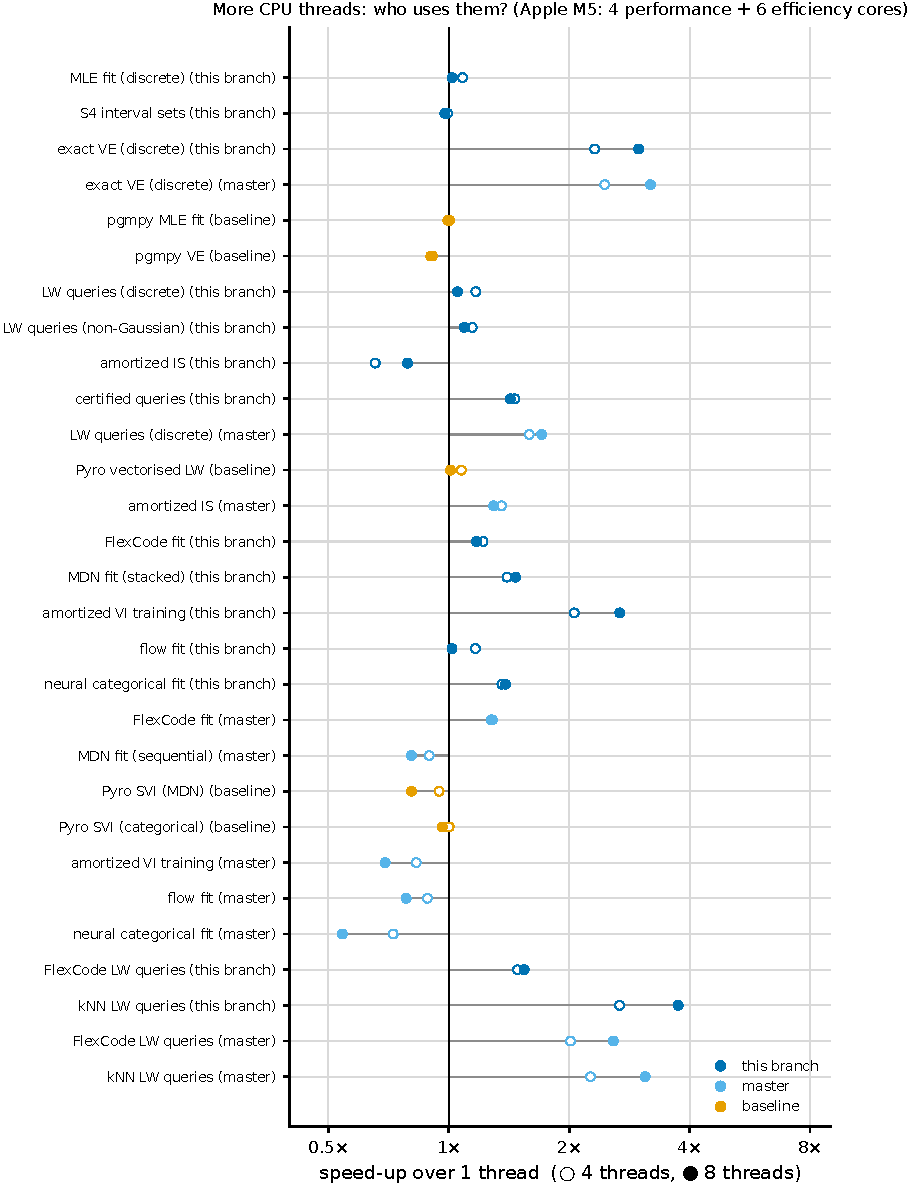
\includegraphics[width=\linewidth]{r3_1_threads_speedup.pdf}
\caption{Speed-up from 1 to 8 CPU threads.}
\end{figure}
\tabthree{r3threads}
Threads help where the work is a few large tensor operations: exact VE ($3.0\times$), kNN
likelihood weighting ($3.75\times$), amortized VI training ($2.7\times$; master was slower with
more threads, $0.69\times$). They do little for MLE fitting, S4 sets and most samplers, whose
cost is a Python loop over nodes.
\begin{figure}[H]\centering
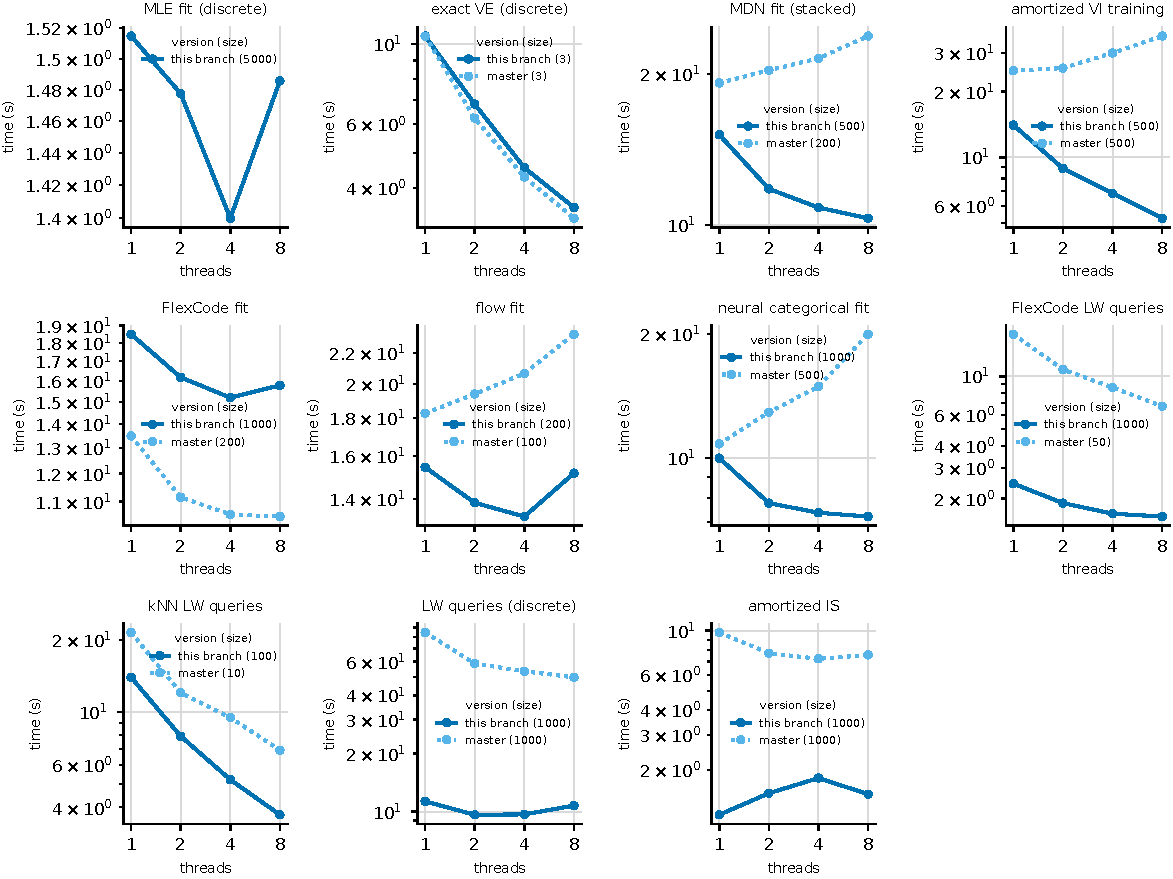
\includegraphics[width=0.8\linewidth]{r3_2_threads_branch_vs_master.pdf}
\caption{Threads: this branch vs master at the same sizes.}
\end{figure}

\subsection{GPU}
\begin{figure}[H]\centering
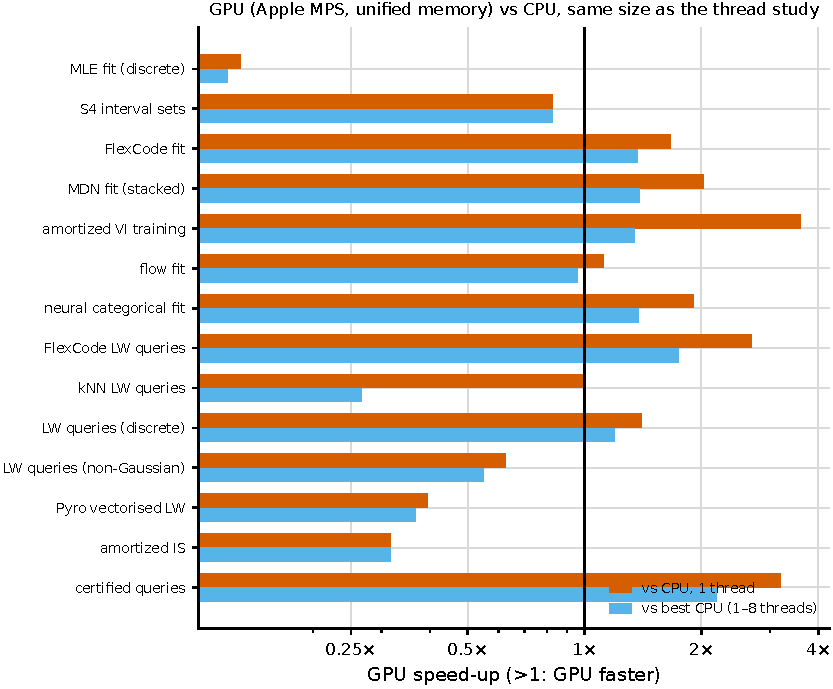
\includegraphics[width=\linewidth]{r3_3_gpu.pdf}
\caption{GPU (Apple MPS) vs CPU.}
\end{figure}
\tabthree{r3gpu}
The GPU helps batched neural work (amortized VI $3.6\times$, certified queries $3.2\times$,
FlexCode LW $2.7\times$) and hurts small or loop-bound work (MLE fit $0.13\times$, amortized IS
$0.32\times$). Exact VE on MPS answered fewer queries: MPS tensors have at most 16 dimensions,
and its allocator does not reuse freed blocks within a query, so the memory guard is stricter.
Round 4 removes the first limit.

\subsection{Frontier: the largest graph finished}
\begin{figure}[H]\centering
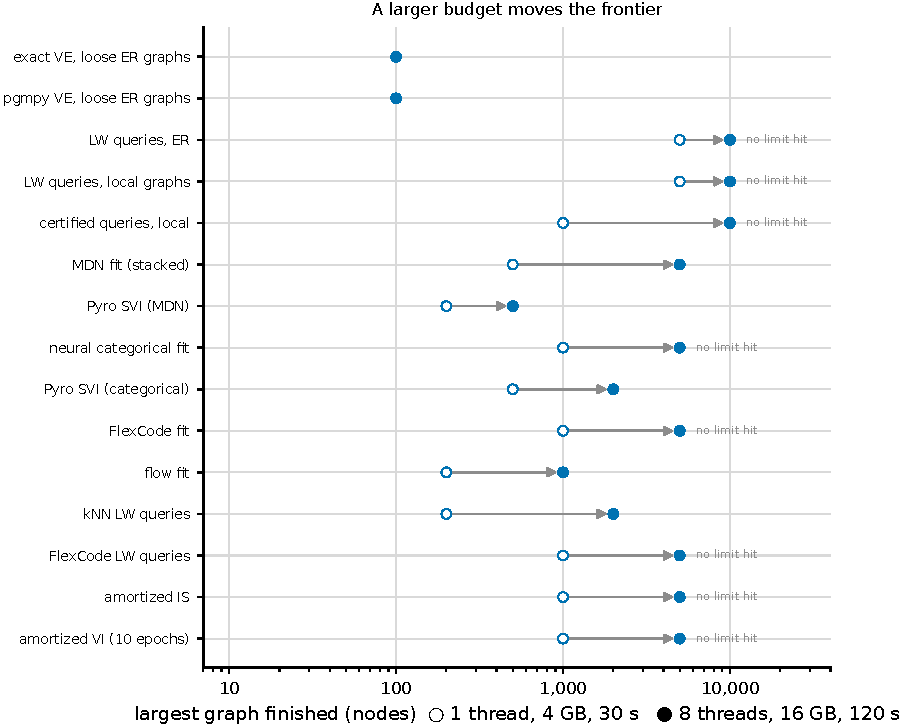
\includegraphics[width=\linewidth]{r3_4_frontier.pdf}
\caption{Largest graph finished, reference budget (1 thread, 4\,GB, 30\,s) vs large budget (8 threads, 16\,GB, 120\,s).}
\end{figure}
\tabthree{r3frontier}
A $4\times$ budget moves the frontier by 2--$10\times$ in nodes for every method \emph{except}
exact VE, whose limit is the elimination width, not the number of nodes.

\subsection{Exact VE: width, not size}
\begin{figure}[H]\centering
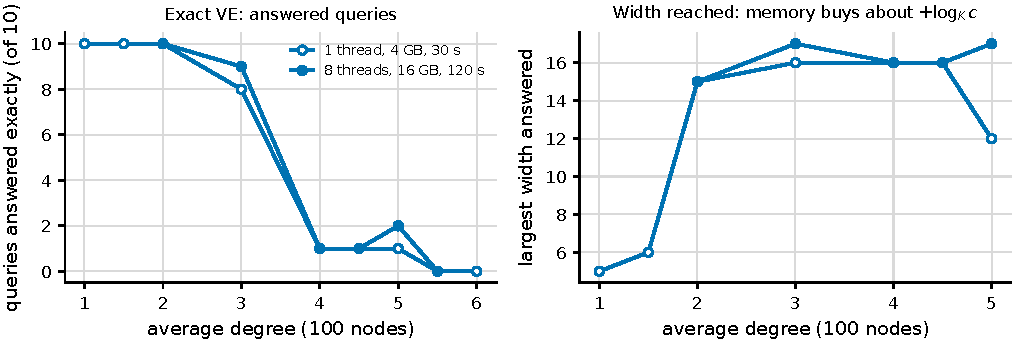
\includegraphics[width=0.8\linewidth]{r3_5_ve_width.pdf}
\caption{Exact VE on denser graphs (100 nodes, $K=3$).}
\end{figure}
\tabthree{r3vewidth}
With $4\times$ the memory the largest width answered goes from 16 to 17, as predicted:
$\log_3 4 \approx 1.26$. Memory alone cannot rescue dense graphs. This is the motivation for
conditioning (round 4).

\subsection{Particles}
\begin{figure}[H]\centering
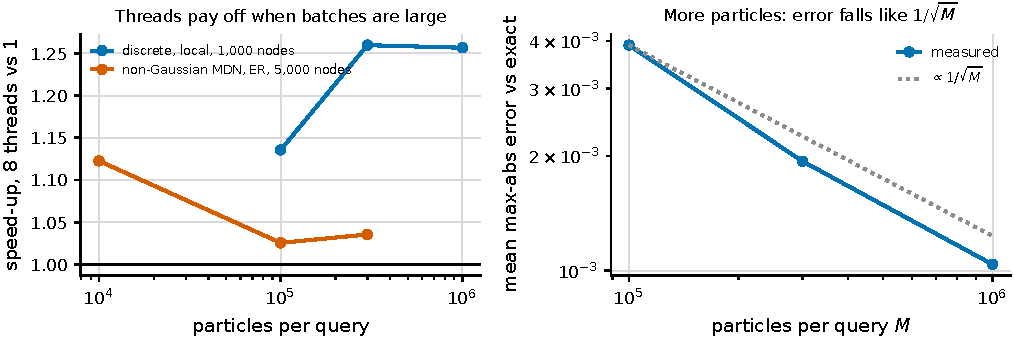
\includegraphics[width=0.8\linewidth]{r3_6_particles.pdf}
\caption{Likelihood weighting with more particles.}
\end{figure}
\tabthree{r3particles}
Time buys accuracy as theory says: error $0.0039\to0.0019\to0.0010$ for $10^5\to3\cdot10^5\to10^6$
particles ($\propto1/\sqrt{M}$). Threads give only $1.26\times$ even at $10^6$ particles: the
sampler loops over nodes in topological order, and each step is too small to split well.
Running \emph{queries} in parallel would use the workers better (next steps).

\section{Round 4: three opt-in options that turn budget into answers}
Nothing changes by default: every option below must be asked for. The default
\code{certified\_query} path gives bit-identical results (test), and plain VE still raises
\code{OutOfMemoryError} when a query does not fit.
\begin{table}[H]\centering\small
\caption{Round-4 options (commits \code{f6d19fe}, \code{3a5ff28}, \code{870d2ab}).}
\resizebox{\linewidth}{!}{%
\renewcommand{\arraystretch}{1.15}\begin{tabular}{>{\raggedright\arraybackslash}p{0.27\linewidth}>{\raggedright\arraybackslash}p{0.33\linewidth}>{\raggedright\arraybackslash}p{0.34\linewidth}}\toprule
option & what it does & guarantee \\ \midrule
\code{TensorVariableElimination(}\allowbreak\code{on\_oom="condition")}; \code{HybridRouter(}\allowbreak\code{fallback="condition")}; \code{conditioned\_query(...)} & when VE does not fit memory (or, on MPS, needs more than 16 tensor dimensions), clamp a greedy cutset $C$ (Bidyuk \& Dechter 2007) and sum the exact VE answers over its instantiations, many at once as rows of one batched elimination & exact (equal to VE to $10^{-7}$ in tests down to 1\% of the memory VE needs); refuses beyond \code{max\_conditioning} instantiations, and the router then falls back to LW \\
\code{certified\_query(...,}\allowbreak\code{ time\_budget\_s=, target\_width=)} & anytime certified sampling: checkpoints $n_j=n_0 2^{j-1}$ at level $\delta_j=\delta/(j(j+1))$; the answer is the intersection of all checkpoint intervals & all checkpoint intervals hold together with probability $\ge 1-\delta$ (union bound; the simplest ``stitching'' of Howard et al.\ 2021), whatever the stopping rule; never wider with more time \\
\code{certified\_query(...,}\allowbreak\code{ collapse="auto"|[vars])} & collapsed (cutset) sampling: sample only the ancestral closure of a cutset, compute the rest exactly (K\&F §12.4) & same certificate (per-particle statistics stay in $[0,W]$, K\&F Eq.\ 12.11); exact when nothing is left to sample \\
\code{conditioned\_query(...,}\allowbreak\code{ time\_budget\_s=}\allowbreak\code{ or enumerate\_limit=)} & bounded conditioning: enumerate instantiations in order of prior frequency; unseen mass $U$ bounds the rest: $[A_y/(A+U),\,(A_y+U)/(A+U)]$ (K\&F §12.5, Eqs.\ 12.35--36) & sound with probability 1 (deterministic); exact when all instantiations are enumerated \\ \bottomrule
\end{tabular}}
\end{table}
\textbf{Devices.} All options run on CPU, CUDA and MPS. On MPS the planner respects the 16-dimension
and $2^{27}$-element tensor limits and keeps float64 accumulators on the CPU. Tests: the full unit
suite passes on the Mac (CPU and MPS); the inference tests pass on the server (NVIDIA TITAN X
Pascal 12\,GB, torch 2.7.1+cu126; only MPS-specific tests skip).

\textbf{Machines.} CPU and CUDA results come from the server (20 cores, 125\,GB, TITAN X); MPS
results from the Mac (idle-gated). E1: 100-node ER graphs, $K=3$, 10 queries with 5 evidence
variables, average degree 3, 4.5 and 6, memory budgets 1, 4, 16\,GB (10\,GB on CUDA); at most
$10^6$ instantiations and 20\,s per query (a slower query is stopped and its time projected
from its measured rate). E2: 4\,GB, time budgets 0.25--16\,s. E3: 1\,GB, 1--64\,s.

\subsection{E1. Conditioning: time and workers now buy exact answers}
\begin{figure}[H]\centering
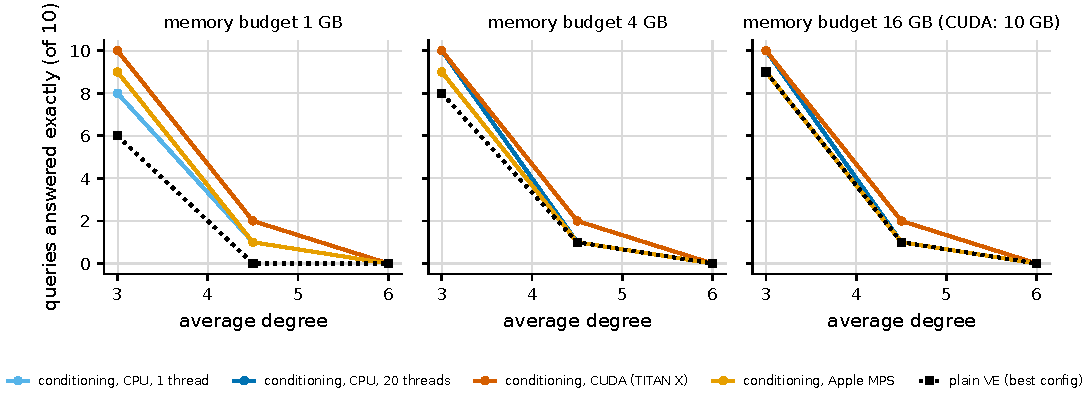
\includegraphics[width=\linewidth]{r4_1_exact_answered.pdf}
\caption{Queries answered exactly within 20\,s, by memory budget and graph density.}
\end{figure}
\begin{figure}[H]\centering
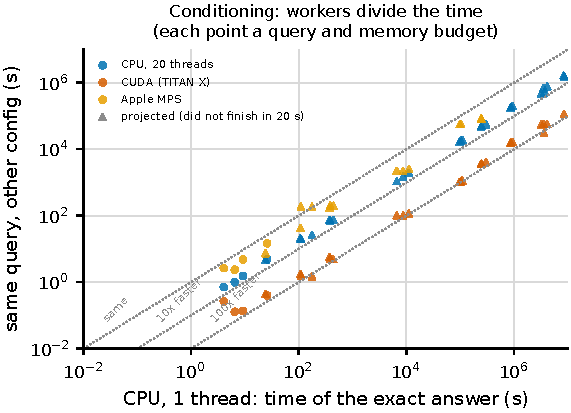
\includegraphics[width=0.62\linewidth]{r4_2_conditioning_speedup.pdf}
\caption{Each point is one conditioned query: its time on another configuration against its time
on 1 CPU thread (triangles: projected from the measured rate). Workers divide the time almost
uniformly, because instantiations are independent rows of one batched elimination.}
\end{figure}
\begin{figure}[H]\centering
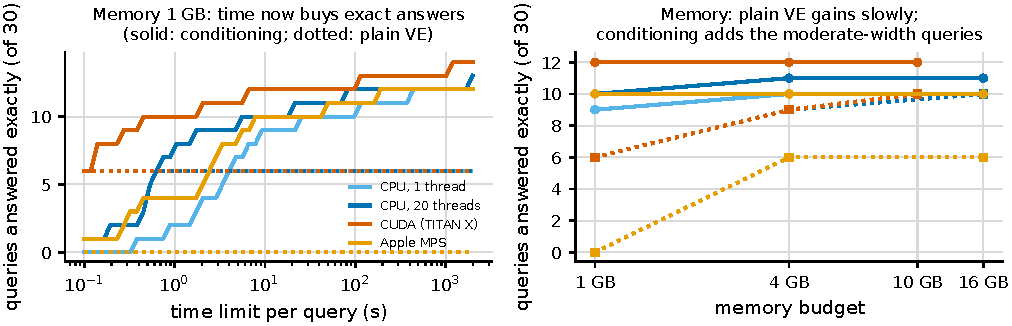
\includegraphics[width=\linewidth]{r4_3_budget_buys_answers.pdf}
\caption{Left: at 1\,GB, the number of exact answers grows with the time limit (solid), while
plain VE (dotted) is flat; beyond 20\,s the times are projected from the measured rate. Right: by memory budget, within 20\,s.}
\end{figure}
\tabfour{r4e1}
\textbf{Reading.} (1) At 1\,GB, 30 queries: plain VE answers 6 (MPS: 0). Conditioning answers
9 within 20\,s on 1 CPU thread, 10 on 20 threads, 12 on CUDA and 10 on MPS. With 1 hour per
query (projected), the total reaches 12--14. (2) More memory means a smaller cutset but
does not add exact answers beyond the degree-3 graphs. (3) On MPS, conditioning also removes
the 16-dimension crash and the stricter memory guard (the MPS allocator does not reuse freed
blocks within a query, so the guard charges more): 0/10 $\to$ 9/10 at 1\,GB. (4) Degree
$\ge4.5$ is out of reach: this is the exponential cost of K\&F Thm 9.11, not an implementation
limit.

\subsection{E2. Anytime certified sampling}
\begin{figure}[H]\centering
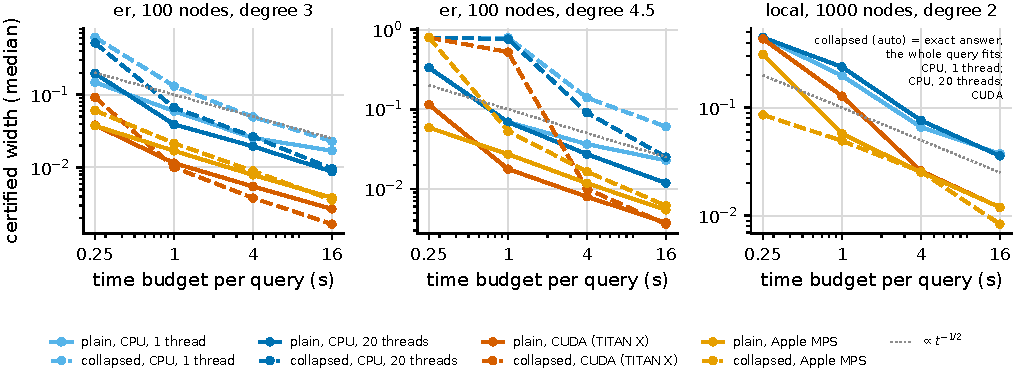
\includegraphics[width=\linewidth]{r4_4_certified_anytime.pdf}
\caption{Median certified width (95\%, all classes) by time budget, 10 queries per problem.}
\end{figure}
\tabfour{r4e2}
\textbf{Reading.} (1) Plain anytime sampling: the width falls like $1/\sqrt{t}$ on every
configuration (dotted guide), and the GPU reaches a given width 4--$16\times$ sooner than CPU. Coverage was
584/584 runs where the exact answer is known (plain and collapsed). (2) Collapsed sampling: on the sparse 1000-node graph,
\code{"auto"} finds that the whole query fits and returns the exact answer on CPU and CUDA (on MPS the stricter
memory model leaves a small cutset: still the narrowest interval at 16\,s). On the dense ER graphs it pays
only on the GPU and at larger budgets (CUDA, degree 3, 16\,s: $0.0017$ vs $0.0027$). On CPU it is
1--$2.6\times$ wider than plain sampling. The first version of the \code{"auto"} rule sized the
cutset for one particle and never reached a checkpoint on dense graphs (width 1); the rule now
sizes it for a batch of particles (commit \code{870d2ab}); the table shows the rerun.
Recommendation: keep \code{collapse=None} as the default, and use \code{"auto"} on accelerators or when the
query is close to fitting.

\subsection{E3. Bounded conditioning}
\begin{figure}[H]\centering
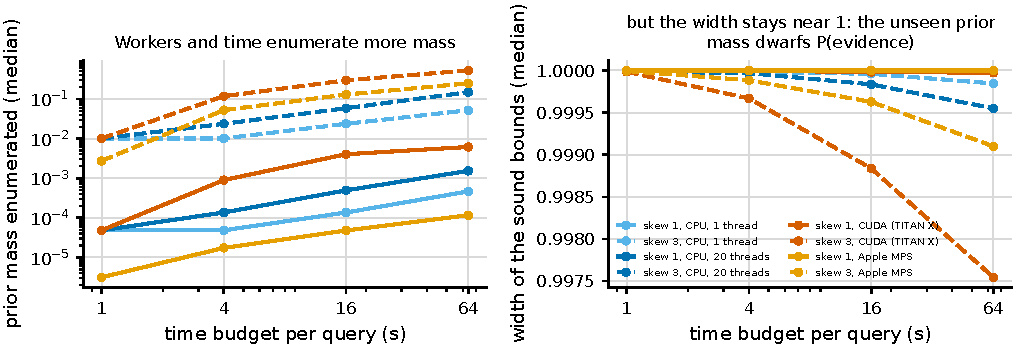
\includegraphics[width=\linewidth]{r4_5_bounded_conditioning.pdf}
\caption{Bounded conditioning (degree 4.5, 1\,GB, 5 queries; skew 3 multiplies the CPT logits by 3).}
\end{figure}
\tabfour{r4e3}
\textbf{Reading.} Workers and time enumerate more prior mass: up to 52\% on CUDA with skewed CPTs
in 64\,s. The bounds are sound, but their width $U/(A+U)$ stays near 1. The covered evidence mass
$A=\sum_{c\in S}P(c,e)$ is at most $P(e)$, here about $10^{-2}$--$10^{-3}$ with 5 evidence
variables, while the unseen mass is $U = 1-\sum_{c\in S}P(c)$. So the width falls only when
$U\lesssim P(e)$. This matches the condition in K\&F §12.5: bounded conditioning works when a
few instantiations carry most of the mass. One query in five (a small cutset) is exact.

\section{Limits and next steps}
\label{sec:next}
\begin{itemize}
\item \textbf{The exponential wall stays.} Conditioning turns workers and time into exact
answers only for moderate widths: the largest cutsets answered within 20\,s have 5 variables
($3^5=243$ instantiations, about 6\,s on CUDA or MPS); with 10 or more, projected times are
$10^3$\,s and up, even on the GPU. Beyond that, the anytime certified interval is the right output: it uses every worker,
and its guarantee is explicit.
\item \textbf{Run queries in parallel.} LW gains only $1.26\times$ from threads (round 3,
per-node loop). A query-parallel executor (one query per worker) would use the cores fully for
batches of queries. This is not implemented yet.
\item \textbf{Tighter bounded conditioning} (ours, sketch, not implemented). For an unseen $c$,
$P(c,e)\le W\,Q(c)$, where $Q$ is the forward-sampling law with the evidence clamped, and
$W=\prod_{e_i}\max_{pa}P(e_i\mid pa)$ (the LW weight bound, K\&F Eq.\ 12.11). Replacing
$U=1-\sum_S P(c)$ with $U_e=W(1-\sum_S Q(c))$ is still sound with probability 1. It is tighter
by a factor of about $W/P(e)$ in the required coverage, and enumerating in order of $Q$ matches the
bound. To be checked with \code{koller\_claude} before implementing.
\item \textbf{Portfolio fitting} (\code{fit} over table / MDN / flow candidates): the cost is the
sum of the candidates. Successive halving (Hyperband, Li et al.\ 2018) and parallel candidates
are the budget-aware versions; not implemented in this round.
\item \textbf{Timing caveats.} Mac timings (round 3 and MPS) were taken on a shared machine with
an idle gate, so they are conservative. Server timings are clean. Projected times assume a
constant rate per instantiation.
\end{itemize}

\section*{References}
\begin{itemize}\small
\item D.\ Koller, N.\ Friedman. \emph{Probabilistic Graphical Models.} MIT Press, 2009 (§9.5 conditioning; §12.4 collapsed particles; §12.5 bounded conditioning).
\item B.\ Bidyuk, R.\ Dechter. Cutset sampling for Bayesian networks. \emph{JAIR} 28, 2007. \url{https://arxiv.org/abs/1110.2740}
\item E.\ Horvitz, H.\ J.\ Suermondt, G.\ Cooper. Bounded conditioning: flexible inference for decisions under scarce resources. \emph{UAI} 1989, pp.\ 182--193. \url{https://arxiv.org/abs/1304.1512}
\item S.\ R.\ Howard, A.\ Ramdas, J.\ McAuliffe, J.\ Sekhon. Time-uniform, nonparametric, nonasymptotic confidence sequences. \emph{Ann.\ Statist.} 49(2), 2021. \url{https://arxiv.org/abs/1810.08240}
\item I.\ Waudby-Smith, A.\ Ramdas. Estimating means of bounded random variables by betting. \emph{JRSS B} 86(1), 2024. \url{https://arxiv.org/abs/2010.09686}
\item L.\ Li, K.\ Jamieson, G.\ DeSalvo, A.\ Rostamizadeh, A.\ Talwalkar. Hyperband. \emph{JMLR} 18, 2018. \url{https://arxiv.org/abs/1603.06560}
\item M.\ J.\ Kochenderfer et al. \emph{Algorithms for Validation.} MIT Press, 2026 (Ex.\ 7.3, p.\ 196).
\end{itemize}

\section*{Reproduce}
\begin{verbatim}
bash benchmarks/scaling/r3_rerun.sh && python benchmarks/scaling/r3_analyze.py
CONFIGS="cpu:1 cpu:20 cuda:4" bash benchmarks/scaling/r4.sh     # server
CONFIGS="mps:1" R=benchmarks/scaling/results/mac bash benchmarks/scaling/r4.sh
python benchmarks/scaling/r4_budget.py e2 --modes collapsed ...  # after 870d2ab
python benchmarks/scaling/r4_merge.py results server mac
python benchmarks/scaling/r4_analyze.py
cd benchmarks/scaling/report && tectonic -X compile report_r3.tex
\end{verbatim}
\end{document}
